\section{From photograph to plywood}
\label{sec:fabrication}

The photograph supplies the printed image and can suggest the perimeter.
Inside that perimeter, fixed figures reserve space before the surrounding
pieces grow. Figure~\ref{fig:production-studies} follows the geometry through
three decisions that affect the physical puzzle.

\begin{figure}[!ht]
\centering
\begin{minipage}{.98\linewidth}
\textbf{(a) Find an outline.}
Nervous System credits rembg for its Magic Shape feature~\cite{magicshape}.
In the archived replay, U\({}^2\)-Net takes a \(320\times320\) RGB image, fuses
predictions at six scales and returns a foreground mask~\cite{u2net}. The red
line below traces the largest outer contour at a mask value of 128. On this
one photograph, the full and compact models matched the upstream reference
mask with intersection-over-union scores of 0.99916 and 0.97213. The studio
has not published how it converts its prediction into a cut perimeter.
\par\smallskip
{\centering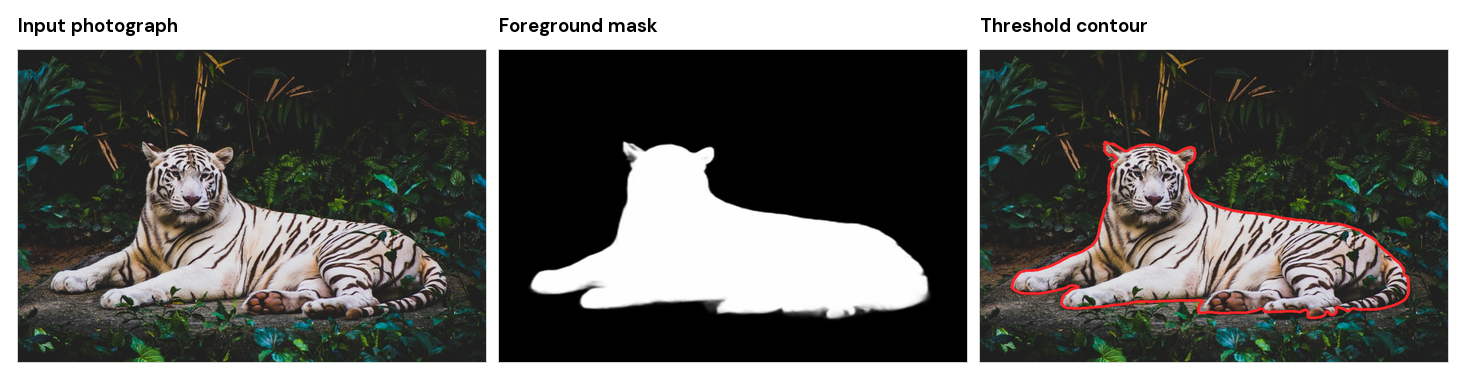
\includegraphics[width=.91\linewidth]{mask-flow.png}\par}
\medskip
\textbf{(b) Reserve the figure pieces.}
For \emph{Herding Cats}, the studio used Deepnest to fit cat silhouettes inside
a larger cat outline, then adjusted their placement by hand~\cite{herdingcats}.
The surrounding pieces grow through the gaps. In the published Dendrite
method, fixed figures act as reflecting boundaries during initialization~\cite{puzzle2012}.
\par\smallskip
{\centering\plate{fixed-figures}{.89}\par}
\medskip
\textbf{(c) Make a cuttable boundary.}
The original Dendrite workflow dilates pieces and removes fragments that pinch
off. Modified marching squares traces the resulting contours. Where a point
lies too close to another edge, local smoothing widens the clearance before
export~\cite{puzzleproject}. The laser follows those paths across the printed
wood. The studio also developed an air-assist nozzle to limit scorching while
cutting its puzzles~\cite{airassist}.
\par\smallskip
{\centering\plate{cut-to-wood}{.78}\par}
\end{minipage}
\caption{The photo, mask and measured contour in (a) use the archived
\href{https://github.com/danielgatis/rembg/blob/332c16b58e0194f0960f9d6cf38746e7be8546b7/examples/animal-1.jpg}{rembg example photograph}.
The schematics show cells meeting a fixed silhouette in (b) and one cut
producing two matching wooden edges in (c).}
\label{fig:production-studies}
\end{figure}
